% !TeX spellcheck = es_ES
\documentclass[12pt, titlepage]{article}
\usepackage[nottoc,notlot,notlof,numbib]{tocbibind}
\usepackage[letterpaper, margin=2.5cm]{geometry}
\usepackage[utf8]{inputenc}
\usepackage[spanish]{babel}
\usepackage{listings}
% imagenes
\usepackage{graphicx} 
\usepackage{float}
% fin imagenes
\usepackage{url}
\usepackage{color}
\usepackage{amsmath}
\usepackage{bm}

\definecolor{dkgreen}{rgb}{0,0.6,0}
\definecolor{gray}{rgb}{0.5,0.5,0.5}
\definecolor{mauve}{RGB}{253,151,31}
\definecolor{deepred}{RGB}{249,38,114}

\lstset{frame=tb,
	language=MATLAB,
	aboveskip=3mm,
	belowskip=3mm,
	showstringspaces=false,
	columns=flexible,
	numbers=left,
	stepnumber=1,
	basicstyle={\small\ttfamily},
	numberstyle=\tiny\color{gray},
	keywordstyle=\color{blue},
	commentstyle=\color{dkgreen},
	stringstyle=\color{mauve},
	breaklines=true,
	breakatwhitespace=true,
	tabsize=2,
	morekeywords={self, append},
	emph={},
	emphstyle=\color{deepred}
}

\title{Reporte}
\author{Barrera Pérez Carlos Tonatihu \\ Profesor: Moreno Armendariz Marco Antonio \\ Redes Neuronales \\ Grupo: 3CM2 }
\begin{document}
    \maketitle
    \tableofcontents
    \newpage
    \section{Introducción}
        Este reporte es sobre tres distintas arquitecturas de redes neuronales, las cuales son: Hamming Perceptron Simple y ADALINE. Se incluye una breve explicación sobre estas arquitecturas el como funcionan y sus diferentes representaciones para que sea fácil de entender.
        \\\\
        Además, se programaron estas tres arquitecturas, sujetas a algunas restricciones para que fuera más sencilla su elaboración, el desarrollo de estos programas fue realizado en \emph{MATLAB} ya que nos proporciona un manejo sencillo de matrices, lo cual es el principal elemento con el que trabajan estas redes neuronales. 
        \\\\
        Para verificar el correcto funcionamiento de los programas se realizaron pruebas con entradas de diferentes tamaños y valores, de igual forma se muestra en pantalla el resultado y una representación gráfica. Para complementar los resultados obtenidos se incluye un análisis de estos.
        \\\\
        Finalmente, tenemos una sección de conclusiones sobre la parte más importante de este reporte.
    \newpage
    \section{Marco teórico}
        \subsection{Hamming}
        La red Hamming es una arquitectura capaz de reconocer patrones binarios. Está formada por dos capas como se muestra en la figura \ref{fig:hamming-diagrama}. La primera capa es una capa de propagación hacia adelante (feedforward en ingles), esto quiere decir que los datos de entrada solamente pueden avanzar de su entrada a la salida de la red nunca en sentido opuesto.
        La expresión correspondiente a esta capa es la siguiente.
        \[ a^1=purelin(W^1p+b^1) \]
        donde $a^1$ es la salida de la capa, $W^1$ es la matriz de pesos, $p$ es el vector de entrada y $b^1$ es el bias.
        \begin{figure}[H]
            \begin{center}
                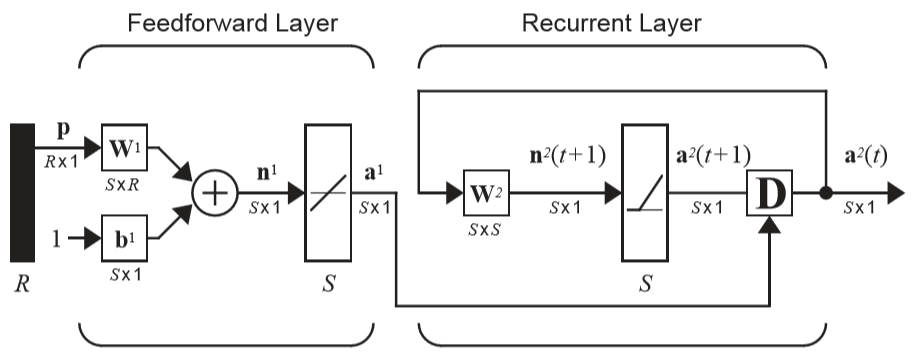
\includegraphics[width=16cm]{img/hamming/diagrama.png}
                \caption{Estructura de la red de Hamming. \cite{libro1}}
                \label{fig:hamming-diagrama}
            \end{center}
        \end{figure}
        En la siguiente capa, la capa recurrente, es donde se realiza una competición con la cual se puede determinar que vector prototipo es el más parecido al vector de entrada.\cite{libro1}
        Es por esto que esta red es de tipo competitiva además de que es de las redes más simples en su categoría.
        Esta capa tiene como expresión matemática a:
        \[\boldsymbol{a^2(t+1) = poslin(W^2a^2(t))}\]
        En esta capa se produce una inhibición lateral, esto quiere decir que la salida de cada neurona tiene un efecto inhibitorio sobre el resto de las neuronas lo cual se ve reflejado en el funcionamiento de la red donde a medida que avanza el valor de alguna neuronas disminuye más lento que el resto. \cite{libro1} 
        
        La construcción de una red de Hamming que reconozca un grupo de vectores prototipo es la siguiente:
        \begin{enumerate}
            \item Si tenemos un conjunto de vectores prototipo como el siguiente.
            \[ \left\lbrace \boldsymbol{p_1, p_2, ..., p_Q} \right\rbrace  \]
            La transpuesta de estos vectores sirven para llenar la matriz de pesos de la primera capa $W^1$ de la siguiente forma.
            \[\boldsymbol{ W^{1}} = \left[\begin{array}{c}\boldsymbol{p^{T}_1}\\\boldsymbol{ p^{T}_2}\\ \vdots \\ \boldsymbol{p^{T}_Q}\end{array}\right]  \]
            \item Por otro lado el bias es llenado con el tamaño $R$ de los vectores prototipo, es decir,
            \[ b^{1} = \left[\begin{array}{c}R\\ R\\ \vdots \\ R\end{array}\right] \]
            \item Para la siguiente capa debido a que es una capa recurrente debemos de inicializar la capa recurrente con el valor de salida de la capa feedforward, es decir, $\boldsymbol{a^2(0) = a^1}$, esto con el fin de poder obtener los siguientes valores de la forma $\boldsymbol{a^2(t+1) = poslin(W^2a^2(t))}$.
            \item Lo siguiente es llenar la matriz de pesos de la segunda capa en donde los elementos en la diagonal de la matriz tendrán valores de uno y el resto serán valores pequeños negativos.
            \[ w^2_{i,j} = \begin{cases} 1 & i=j \\-\epsilon & \text{en otro caso} \end{cases} \]
            El valor de épsilon se obtiene por la siguiente formula: $ 0 < \epsilon <\frac{1}{S-1}$ donde $S$ es el número de neuronas
            \item Finalmente, solo se tiene que introducir un vector en la entrada de la primera capa, propagar hacia adelante y utilizar la recurrencia de la segunda capa hasta que solo una salida de esta capa tenga un valor positivo, el indice de la salida indica que vector prototipo reproduce dicha salida.
        \end{enumerate}
    \newpage
        \subsection{Perceptron}
        El perceptron fue desarrollado en los años cincuenta por un grupo de investigadores entre los que estaba Frank Rosenblantt, la principal característica de esta red es que utiliza un algoritmo de aprendizaje supervisado esto quiere decir que se le tiene que dar ejemplos de como operar (conjunto de entrenamiento), este conjunto de entrenamiento tiene la siguiente forma:
        \[ \left\lbrace \boldsymbol{p_1, t_1}\right\rbrace , \left\lbrace \boldsymbol{p_2, t_2}\right\rbrace , ... , \left\lbrace \boldsymbol{p_Q, t_Q}\right\rbrace  \]
        en donde cada par esta formado por un vector de entrada $\boldsymbol{p_q}$ y un vector objetivo $\boldsymbol{t_q}$ que es la salida correspondiente a dicho vector de entrada. \cite{libro1}
        Además, la arquitectura del perceptron es la siguiente:
        \begin{figure}[H]
            \begin{center}
                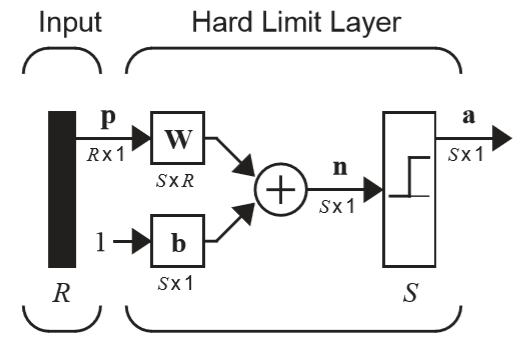
\includegraphics[width=8cm]{img/perceptron/perceptron.png}
                \caption{Arquitectura de un perceptron simple. \cite{libro1}}
                \label{fig:perpectron-diagrama}
            \end{center}
        \end{figure}
        Debido a que utiliza una función \emph{hardlim} la salida de la red solo puede tener dos posibles valores el cual esta definido por $\boldsymbol{a = hardlim(Wp+b)}$. El hecho de que solo tenga dos valores es lo que nos permite establecer una frontera de decisión entre dos clases como la de la figura \ref{fig:frontera}, esto en consecuencia de que cada neurona puede clasificar 2 diferentes clases.
        \begin{figure}[H]
            \begin{center}
                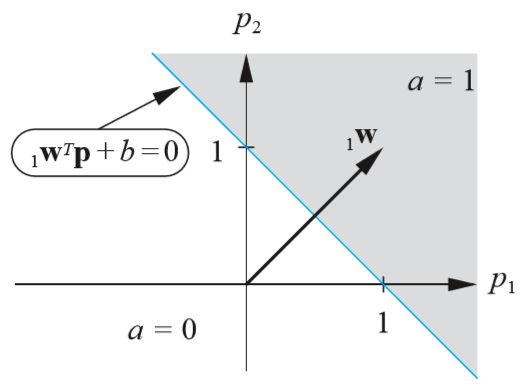
\includegraphics[width=8cm]{img/perceptron/frontera.png}
                \caption{Ejemplo de una frontera de decisión. \cite{libro1}}
                \label{fig:frontera}
            \end{center}
        \end{figure}
        Dicha frontera es determinada por un valor de entrada para el cual la salida de la red es 0, es decir,
        \[\boldsymbol{Wp+b} = 0 \]
        Como se menciono antes, el perceptron utiliza una regla de aprendizaje que se basa en la modificación de los pesos y bias con base a un error a lo largo de la propagación hacia adelante que se realiza. 
        Para lograr esto se sigue el siguiente algoritmo.
        \begin{enumerate}
            \item Se tiene el conjunto de entrenamiento
            \[ \left\lbrace \boldsymbol{p_1, t_1}\right\rbrace , \left\lbrace \boldsymbol{p_2, t_2}\right\rbrace , ... , \left\lbrace \boldsymbol{p_Q, t_Q}\right\rbrace\]
            \item Se inicializan los valores de $\boldsymbol{W}$ y $\boldsymbol{b}$ con valores aleatorios pequeños.
            \item Procedemos a hacer la propagación hacia adelante de un vector prototipo, es decir, evaluamos un $\boldsymbol{p_Q}$ en nuestra red de la forma.
            \[ \boldsymbol{a = hardlim(Wp_Q+b)} \]
            \item Lo siguiente es obtener el error comparando el valor objetivo asociado a dicho vector prototipo con la salida producida por la red
            \[ \boldsymbol{e=t-a} \]
            \item A continuación aplicamos el aprendizaje correspondiente al bias y matriz de pesos de nuestra red. Es decir, el nuevo valor de nuestra matriz de pesos sera igual al valor actual más el producto del error obtenido en el paso por la transpuesta del vector de entrada que se utilizo.
            \[ \boldsymbol{W^{nueva} = W^{vieja} + ep^{t}} \]
            Para el caso del bias tenemos algo similar solo que el nuevo valor de $\boldsymbol{b}$ sera igual al valor actual más el error producido.
            \[ \boldsymbol{b^{nueva} = b^{vieja} + e} \]
            \item Esto se realiza para cada elemento del conjunto de entrenamiento para poder completar una iteración.
            \item Este procedimiento se realiza hasta que cada salida de la red con cada vector de entrada sea igual a su correspondiente objetivo $a_Q = t_Q$ o en el caso de que se alcance un máximo de iteraciones.
        \end{enumerate}
        \newpage
        \subsection{ADALINE}
        La red ADALINE (ADAptive LInear NEuron) es muy similar a al perceptron con la diferencia que la función de transferencia es lineal en lugar de ser escalón esto se puede observar en la figura \ref{fig:adaline-diagrama}, y al igual que el perceptron solo pueden resolver problemas linealmente separables como por ejemplo el problema de la compuerta AND de la figura \ref{fig:AND}. \cite{pagina}
        \begin{figure}[H]
            \begin{center}
                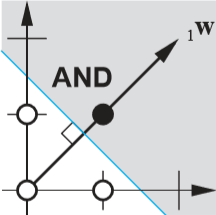
\includegraphics[width=5cm]{img/adaline/AND.png}
                \caption{La compuerta AND es linealmente separable. \cite{libro1}}
                \label{fig:AND}
            \end{center}
        \end{figure}
        Por otro lado un problema linealmente no separable seria el de la figura \ref{fig:XOR} ya que no es posible trazar lineas que funjan como frontera de decision entre las dos clases que tenemos.
        
        Otro aspecto importante de ADALINE es que el algoritmo LMS es mas poderoso que la regla de aprendizaje del perceptron. Esto debido a que la regla de aprendizaje del perceptron garantiza la convergencia a una solución que clasifica los vectores prototipo. Por lo que es sensible al ruido que se produce debido a que estos vectores suelen estar muy cerca de las fronteras de decisión.
        \begin{figure}[H]
            \begin{center}
                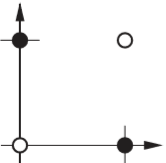
\includegraphics[width=5cm]{img/adaline/XOR.png}
                \caption{La compuerta XOR no se puede separar linealmente. \cite{libro1}}
                \label{fig:XOR}
            \end{center}
        \end{figure}
        Este problema es solucionado con LMS, el cual desplaza las fronteras de decisión lejos de los patrones de entrenamiento esto vuelve a este método más útil y aplicable a otros campos como el procesamiento de señales digital de señales en donde se utiliza para cancelar echo en las lineas telefónicas de larga distancia.
        
        La arquitectura de esta red es la siguiente.
        \begin{figure}[H]
            \begin{center}
                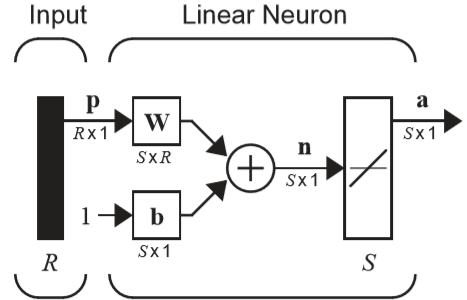
\includegraphics[width=9cm]{img/adaline/arquitectura.png}
                \caption{Arquitectura de la red ADALINE. \cite{libro1}}
                \label{fig:adaline-diagrama}
            \end{center}
        \end{figure}
        Se puede apreciar su similitud con el perceptron incluso en la ecuación que produce la salida de la red, la cual está definida como.
        \[ \boldsymbol{a = purelin(Wp+b)} \]
        Esta red es entrenada por aprendizaje supervisado por lo que utilizamos un conjunto de entrenamiento y el algoritmo LMS que se encarga de ajustar los pesos y bias con el objetivo de minimizar el error medio cuadrático.
        \[ \left\lbrace \boldsymbol{p_1, t_1}\right\rbrace , \left\lbrace \boldsymbol{p_2, t_2}\right\rbrace , ... , \left\lbrace \boldsymbol{p_Q, t_Q}\right\rbrace\]
        El algoritmo es el siguiente. \cite{otro}
        \begin{enumerate}
            \item Inicialización de los pesos y bias de forma aleatoria.
            \item Se aplica un patrón $p_Q$ de entrada.
            \item Se computa una salida lineal utilizando la red.
            \item Se calcula el error cometido por la red para dicho patrón el cual se calcula de la siguiente forma.
            \[\boldsymbol{e_Q = t_Q - a_Q} \]
            donde $\boldsymbol{e_Q}$ es el error, $\boldsymbol{t_Q}$ es el vector objetivo y $\boldsymbol{a_Q}$ es la salida que produce la red.
            \item Se actualizan los pesos y bias utilizando el error obtenido en el paso anterior de la siguiente forma.
            \begin{gather*}
            \boldsymbol{W}(k+1) = \boldsymbol{W}(k) +2\alpha \boldsymbol{e}(k)\boldsymbol{p^T}(k) \\
            \boldsymbol{b}(k+1) =\boldsymbol{b}(k) + 2\alpha \boldsymbol{e}(k)
            \end{gather*}
            donde $\boldsymbol{W}(k+1)$ y $\boldsymbol{b}(k+1)$ son los nuevos valores de nuestros pesos y bias, $\boldsymbol{W}(k)$ y $\boldsymbol{b}(k)$ son los valores actuales, $\alpha$ es un factor de aprendizaje que suele tener valores muy pequeños para evitar modificaciones drásticas en los valores de la red y $\boldsymbol{p^T}(k)$ es la transpuesta de nuestro vector de entrada.
            \item Se repiten los pasos 2 a 5 para todos los patrones de entrenamiento.
            \item Después de esto termina una iteración y se calcula el error cuadrático medio, este error es calculado de la siguiente forma.
            \[ e^2 = \frac{1}{Q} \sum _{i=1}^{Q} e^2_i \]
            Si el error cuadrático medio es un valor reducido aceptable o hemos alcanzado un máximo de iteraciones terminamos el proceso, de lo contrario se vuelve al paso 2.
        \end{enumerate}
    \newpage
    \section{Resultados experimentales}
    En esta sección se puede observar el funcionamiento de las redes antes planteadas y el como trabajan.
        \subsection{Hamming}
        \textbf{Experimento 1}. Es importante señalar que la asignación de valores se realizo a través de un archivo de texto llamado \emph{entrada\_hamming.txt}
        \begin{figure}[H]
            \begin{center}
                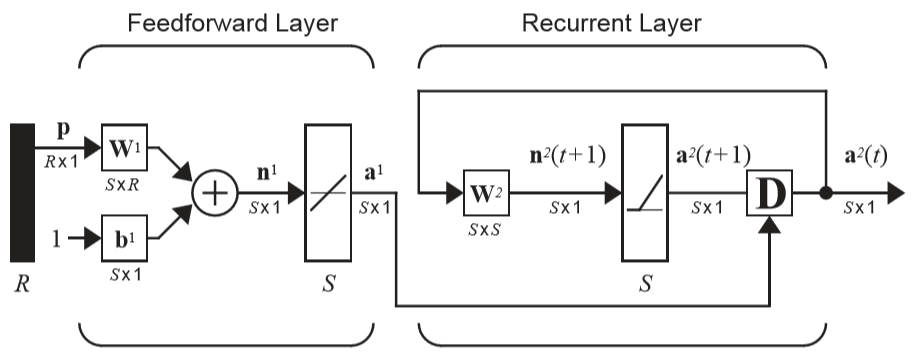
\includegraphics[width=16cm]{img/hamming/diagrama.png}
                \caption{Estructura de la red de Hamming. \cite{libro1}}
                \label{fig:hamming-diagrama2}
            \end{center}
        \end{figure}
        Para hacer la primera prueba sobre la red Hamming se utilizo el siguiente conjunto de vectores prototipo.
        \[ \left\lbrace \boldsymbol{p_1} = \left[\begin{array}{c}-1\\ 1\\ -1\end{array}\right], \boldsymbol{p_2} = \left[\begin{array}{c}-1\\ -1\\ 1\end{array}\right], \boldsymbol{p_3} = \left[\begin{array}{c}1\\ 1\\ -1\end{array}\right], \boldsymbol{p_4} = \left[\begin{array}{c}1\\ -1\\ -1\end{array}\right] \right\rbrace \]
        Y el vector de a clasificar fue el siguiente.
        \[ \boldsymbol{p} = \left[\begin{array}{c}-1\\ 1\\ -1\end{array}\right] \]
        Por lo que la arquitectura definida en la figura \ref{fig:hamming-diagrama2} tiene los siguientes valores.
        \begin{align*}
        R = 3 \implies \boldsymbol{b} = \left[\begin{array}{c}3\\ 3\\ 3\end{array}\right] && S = 4 && \boldsymbol{W} = \left[\begin{array}{c}\boldsymbol{p^{T}_1}\\ \boldsymbol{p^{T}_2}\\ \boldsymbol{p^{T}_3} \\ \boldsymbol{p^{T}_4}\end{array}\right]
        \end{align*}
        Al aplicar estos valores a nuestra red la capa recurrente termino en la iteración 13 y convergió exitosamente a la clase 1 que es la que se esperaba que convergiera.
        %modelo matemático, arquitectura, conjunto de entrenamiento, condición de finalización, valores finales de w y bias
            \begin{figure}[H]
                \begin{center}
                    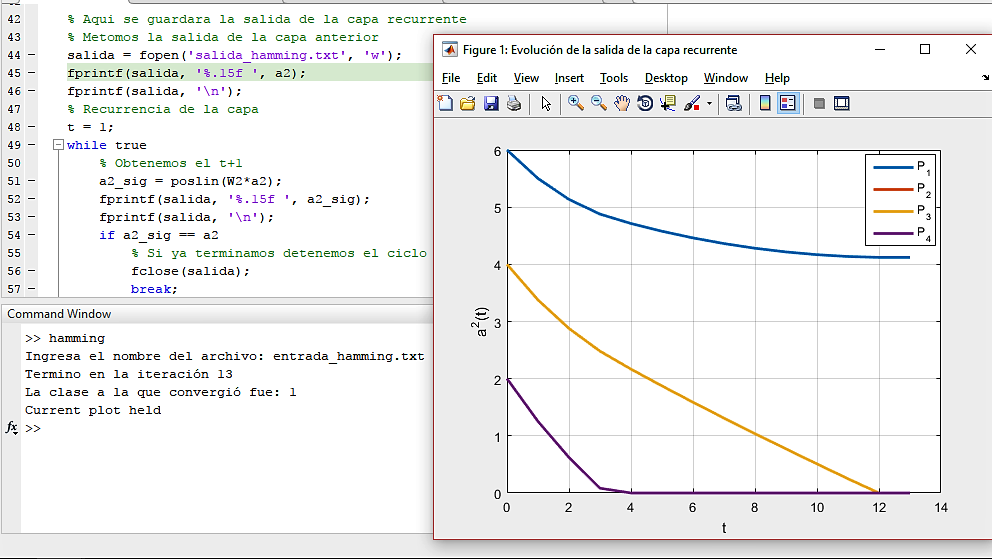
\includegraphics[width=16cm]{img/hamming/hamming1.png}
                    \caption{Prueba 1 de la red Hamming.}
                    \label{fig:hamming1}
                \end{center}
            \end{figure}
       En la figura \ref{fig:hamming1} se puede observar que solo la curva asociada a la neurona 1 de la capa recurrente que corresponde al vector prototipo 1 es la única que tiene un valor distinto de 0.
       \newline
       \textbf{Experimento 2.}
       En esta segunda prueba se utilizo el siguiente conjunto de vectores prototipo.
       \[ \left\lbrace \boldsymbol{p_1} = \left[\begin{array}{c}1\\ -1\\ -1 \\ -1 \end{array}\right], \boldsymbol{p_2} = \left[\begin{array}{c}-1\\ -1\\ -1 \\ 1 \end{array}\right] \right\rbrace \]
       El vector de prueba a clasificar fue el siguiente.
       \[ \boldsymbol{p} = \left[\begin{array}{c}1\\ 1\\ -1 \\ -1\end{array}\right] \]
       Los valores fueron ingresados mediante un archivo de texto llamado \emph{entrada\_hamming2.txt}. Esto dio como resultado que los valores de la red Hamming de la figura \ref{fig:hamming-diagrama2} sean los siguientes.
       \begin{align*}
       R = 4 \implies \boldsymbol{b} = \left[\begin{array}{c}4 \\4\end{array}\right] && S = 2 && \boldsymbol{W} = \left[\begin{array}{c}\boldsymbol{p^{T}_1}\\ \boldsymbol{p^{T}_2}\end{array}\right]
       \end{align*}
            \begin{figure}[H]
                \begin{center}
                    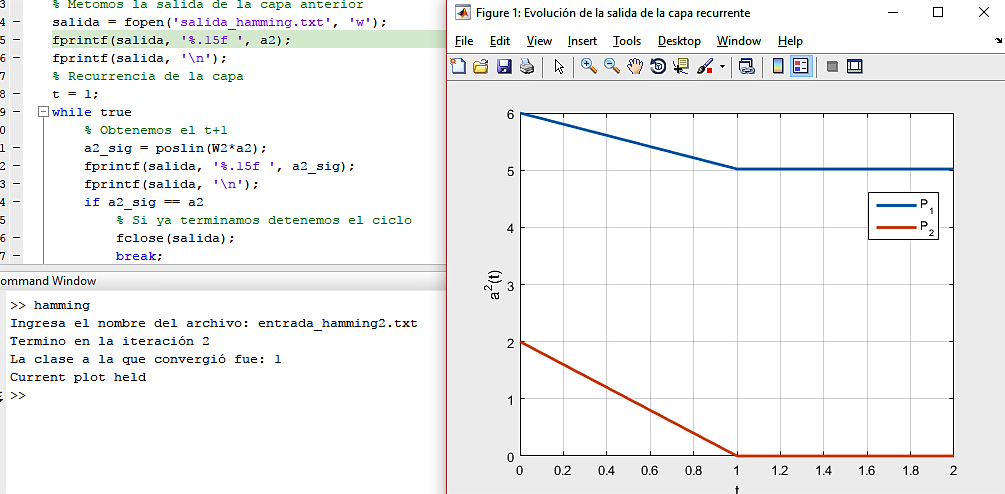
\includegraphics[width=16cm]{img/hamming/hamming2.png}
                    \caption{Prueba 2 de la red Hamming.}
                    \label{fig:hamming2}
                \end{center}
            \end{figure}
        Después del procesamiento de estos datos se pudo clasificar correctamente el vector de entrada, a la red le tomo dos iteraciones logar converger y a la clase a la que convergió fue la 1, esto se puede observar a detalle en la evolución de las salidas de la capa recurrente que se encuentra en la figura \ref{fig:hamming2}.
        \newline
        \textbf{Experimento 3.} En este ultimo experimento se utilizo un archivo llamado \emph{entrada\_hamming3.txt} para poder ingresar los datos a la red. El conjunto de vectores prototipo fue el siguiente.
        \[ \left\lbrace \boldsymbol{p_1} = \left[\begin{array}{c}-1\\ 1\\ 1 \\ 1 \\ 1 \end{array}\right], \boldsymbol{p_2} = \left[\begin{array}{c}-1\\ -1\\ 1 \\ -1 \\ 1 \end{array}\right], \boldsymbol{p_3} = \left[\begin{array}{c}1\\ 1\\ -1 \\ -1 \\ -1 \end{array}\right], \boldsymbol{p_4} = \left[\begin{array}{c}-1\\ -1\\ -1 \\ -1 \\ -1 \end{array}\right], \boldsymbol{p_5} = \left[\begin{array}{c}1\\ 1\\ 1 \\ 1 \\ 1 \end{array}\right] \right\rbrace \]
        El vector de prueba que se utilizo fue.
        \[ \boldsymbol{p} = \left[\begin{array}{c}1\\ -1\\ 1 \\ -1 \\ 1\end{array}\right] \]
        El utilizar estos valores produjo que la arquitectura de la figura \ref{fig:hamming-diagrama2} tuviera los siguientes valores.
        \begin{align*}
        R = 5 \implies \boldsymbol{b} = \left[\begin{array}{c}5 \\5 \\ 5 \\ 5 \\ 5\end{array}\right] && S = 5 && \boldsymbol{W} = \left[\begin{array}{c}\boldsymbol{p^{T}_1}\\ \boldsymbol{p^{T}_2} \\ \boldsymbol{p^{T}_3} \\ \boldsymbol{p^{T}_4} \\ \boldsymbol{p^{T}_5}\end{array}\right]
        \end{align*}
            \begin{figure}[H]
                \begin{center}
                    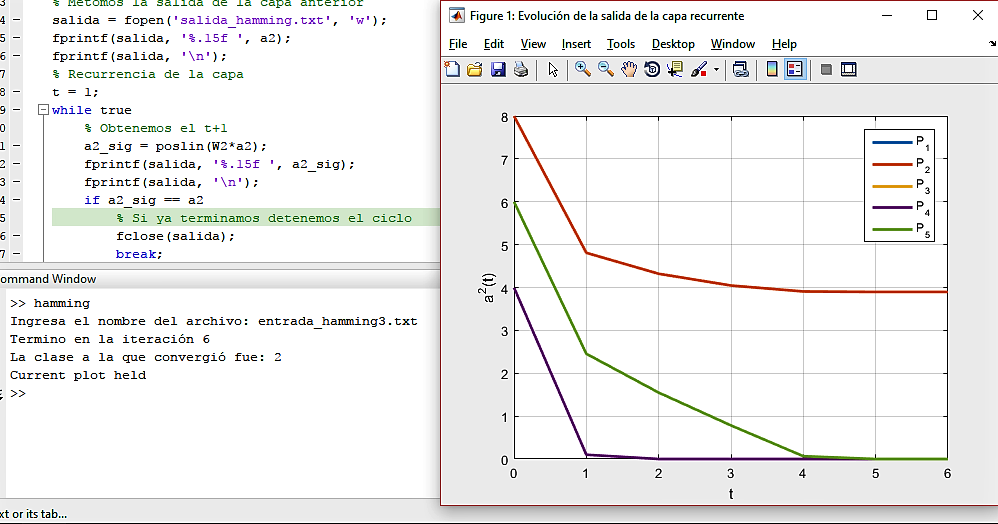
\includegraphics[width=16cm]{img/hamming/hamming3.png}
                    \caption{Prueba 3 de la red Hamming.}
                    \label{fig:hamming3}
                \end{center}
            \end{figure}
        Como se puede observar en la figura \ref{fig:hamming3} la red pudo converger a un resultado satisfactorio en la iteración 6 dando como resultado que el vector de prueba perteneciera a la clase 2 debido a que es la única salida que tiene un valor diferente a 0.
        \newpage
        \subsection{Perceptron}
        \textbf{Experimento 1}
        \textbf{Experimento 2}
        \subsection{ADALINE}
        Los experimentos en ADALINE consistieron se dividieron en dos partes, la primera para pruebas que involucraran bias en donde se introdujo un archivo con el conjunto de entrenamiento al igual que en el perceptron, y por otro lado para la parte en la que no se utilizo el bias sólo se resolvió el problema del codificador en el cual el usuario indica el tamaño del codificador y la red comienza a trabajar como lo haría comúnmente.
        
        Ambos tipos de experimentos incluyen la graficación de la evolución del error por iteración y de los valores de pesos y bias, además de que los valores finales son almacenados en un archivo llamado \emph{resultado\_hora\_fecha.txt}
        \begin{figure}[H]
            \begin{center}
                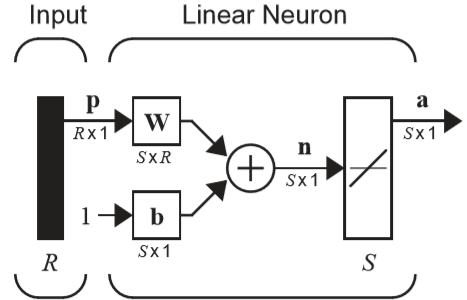
\includegraphics[width=9cm]{img/adaline/arquitectura.png}
                \caption{Arquitectura de la red ADALINE con bias. \cite{libro1}}
                \label{fig:adaline-diagrama2}
            \end{center}
        \end{figure}
            \subsubsection{Con bias}
            \textbf{Experimento 1}
            El conjunto de entrenamiento que se utilizo en este caso fue.
            \[ \left\lbrace \boldsymbol{p_1} = \left[\begin{array}{c} 0\\ 0\end{array}\right], t_1 = -1  \right\rbrace, \left\lbrace \boldsymbol{p_2} = \left[\begin{array}{c} 0\\ 1\end{array}\right], t_2 = -1  \right\rbrace, \left\lbrace \boldsymbol{p_3} = \left[\begin{array}{c} 1\\ 0\end{array}\right], t_3 = -1  \right\rbrace, \left\lbrace \boldsymbol{p_4} = \left[\begin{array}{c} 1\\ 1\end{array}\right], t_4 = 1  \right\rbrace  \]
            El cual corresponde a una compuerta AND de dos entradas. Esto provoco que los valores asociados a nuestra arquitectura de la figura \ref{fig:adaline-diagrama2} fueran los siguientes.
            \begin{align*}
                S=1 && R=2
            \end{align*}
            Además los valores asociados a $\boldsymbol{W}$ y $\boldsymbol{b}$ fueron números aleatorios pequeños. De igual forma se ingresan los valores para el factores de aprendizaje, número máximo de iteraciones y el mínimo error permitido, $\alpha=.03$, $it_{max}=100$, $e_{it}=.1$ respectivamente.
            \begin{figure}[H]
                \begin{center}
                    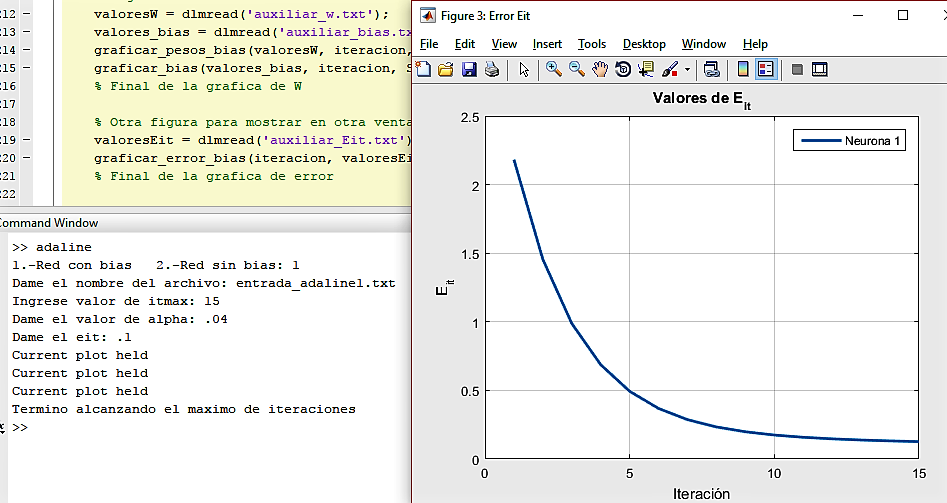
\includegraphics[width=16cm]{img/adaline1/error.png}
                    \caption{Prueba 1 de ADALINE con bias.}
                    \label{fig:adaline1error}
                \end{center}
            \end{figure}
            En la figura \ref{fig:adaline1error} se puede observar que la red llego a un resultado en la iteración 25 debido al criterio de error menor al permitido por iteración como se ve reflejado en la gráfica correspondiente, dando como resultado los siguientes valores para los pesos y bias.
            \begin{align*}
                \boldsymbol{W} = \left[\begin{array}{cc}0.5744 & 0.5956\end{array}\right] && \boldsymbol{b} = -0.9391
            \end{align*}
            Estos valores son almacenados en su respectivo archivo \emph{resultado\_hora\_fecha.txt}, en la figura \ref{fig:adaline1pesos} se puede observar su evolución a lo largo de las 25 iteraciones.
            \begin{figure}[H]
                \begin{center}
                    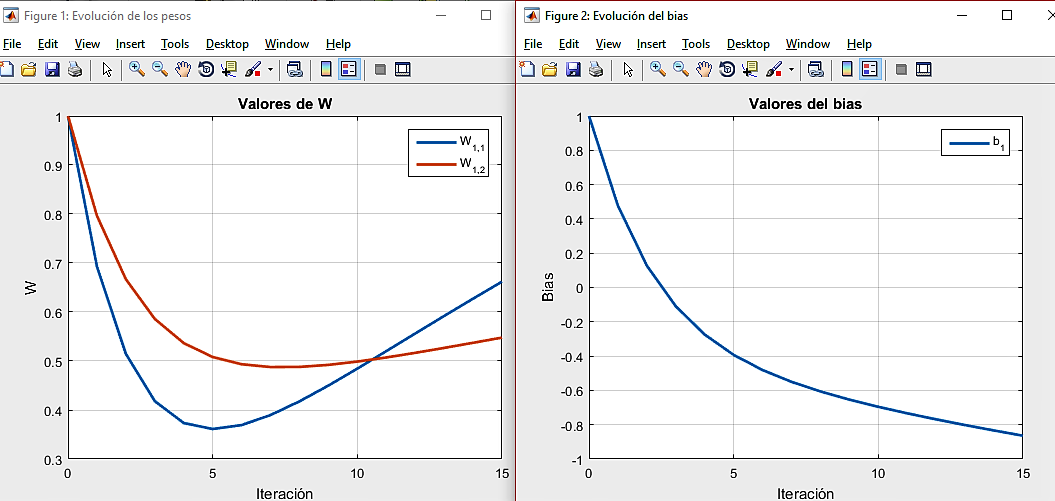
\includegraphics[width=16cm]{img/adaline1/pesosbias.png}
                    \caption{Pesos y bias en esta prueba.}
                    \label{fig:adaline1pesos}
                \end{center}
            \end{figure}
        \textbf{Experimento 2}
        El conjunto de entrenamiento que se utilizo para entrenar a la red fue.
        \[ \left\lbrace \boldsymbol{p_1} = \left[\begin{array}{c} 1\\ 1\end{array}\right], \boldsymbol{t_1} = \left[\begin{array}{c} -1\\ -1\end{array}\right]  \right\rbrace, \left\lbrace \boldsymbol{p_2} = \left[\begin{array}{c} 2\\ 0\end{array}\right], \boldsymbol{t_2} = \left[\begin{array}{c} -1\\ -1\end{array}\right]  \right\rbrace, \left\lbrace \boldsymbol{p_3} = \left[\begin{array}{c} -1\\ -1\end{array}\right], \boldsymbol{t_3} = \left[\begin{array}{c} -1\\ 1\end{array}\right]  \right\rbrace,\]
        
        \[ \left\lbrace \boldsymbol{p_4} = \left[\begin{array}{c} 0\\ -1\end{array}\right], \boldsymbol{t_4} = \left[\begin{array}{c} -1\\ 1\end{array}\right]  \right\rbrace, \left\lbrace \boldsymbol{p_5} = \left[\begin{array}{c} -2\\ 0\end{array}\right],\boldsymbol{t_5} = \left[\begin{array}{c} 1\\ -1\end{array}\right]  \right\rbrace, \left\lbrace \boldsymbol{p_6} = \left[\begin{array}{c} -1\\ 1\end{array}\right], \boldsymbol{t_6} = \left[\begin{array}{c} 1\\ -1\end{array}\right]  \right\rbrace,\]
        
        \[ \left\lbrace \boldsymbol{p_7} = \left[\begin{array}{c} 0\\ 2\end{array}\right], \boldsymbol{t_7} = \left[\begin{array}{c} 1\\ 1\end{array}\right]  \right\rbrace, \left\lbrace \boldsymbol{p_8} = \left[\begin{array}{c} 1\\ 2\end{array}\right], \boldsymbol{t_8} = \left[\begin{array}{c} 1\\ 1\end{array}\right]  \right\rbrace\]
        Es por estos valores que las dimensiones de la red mostrada en la figura \ref{fig:adaline-diagrama2} quedan definidas de la siguiente forma.
        \begin{align*}
            S = 2 && R = 2
        \end{align*}
        Lo cual crea una matriz de pesos de $2x2$ y una matriz de bias de $2x1$ con valores aleatorios pequeños, mientras que los valores de iteración máxima, factor de aprendizaje y error permitido son de nueva cuenta introducidos manualmente de la forma $it_{max}=20$, $\alpha=0.04$,  $e_{it}=0.1$ respectivamente (véase figura \ref{fig:adaline2error}).
        \begin{figure}[H]
            \begin{center}
                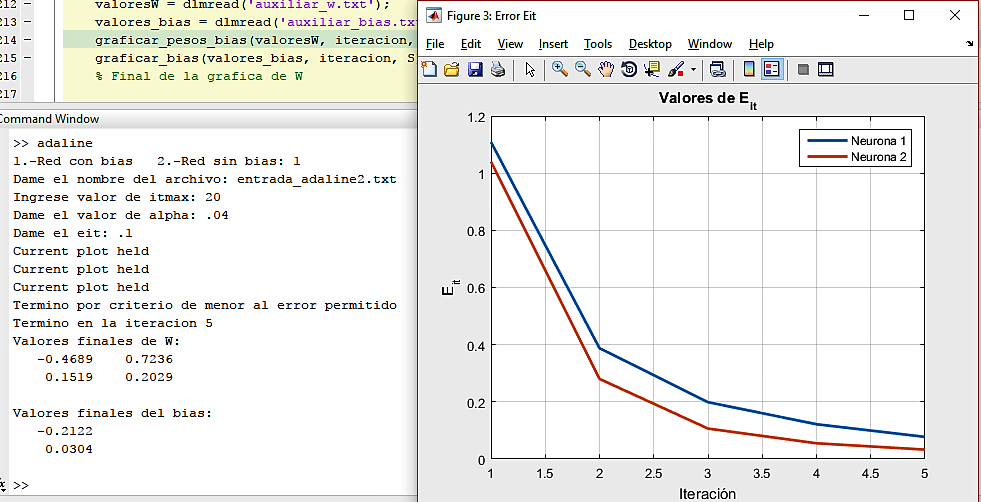
\includegraphics[width=16cm]{img/adaline2/error.png}
                \caption{Prueba 2 de ADALINE con bias.}
                \label{fig:adaline2error}
            \end{center}
        \end{figure}
        En esta ocasión la red convergió en la iteración 5 debido al criterio de menor al error permitido reflejado en la figura \ref{fig:adaline2error} para cada una de las neuronas que componen esta red. Los valores finales de pesos y bias se almacenaron en su correspondiente archivo de salida con los valores.
        \begin{align*}
            \boldsymbol{W} = $\left[\begin{array}{cc}-0.4648&amp; 0.7236\\ 0.1519&amp; 0.2029\end{array}\right]$&& \boldsymbol{b} = $\left[\begin{array}{c}-0.2122\\ 0.0304\end{array}\right]$
        \end{align*}
        \begin{figure}[H]
            \begin{center}
                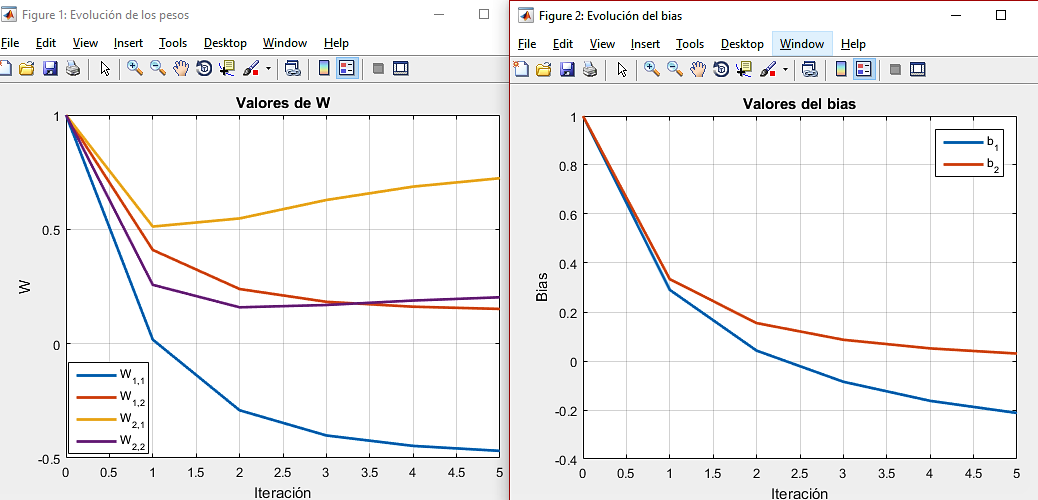
\includegraphics[width=16cm]{img/adaline2/pesosbias.png}
                \caption{Pesos y bias en esta prueba.}
                \label{fig:adaline2pesos}
            \end{center}
        \end{figure}
            \subsubsection{Sin bias}
            \textbf{Experimento 1}
            \begin{figure}[H]
                \begin{center}
                    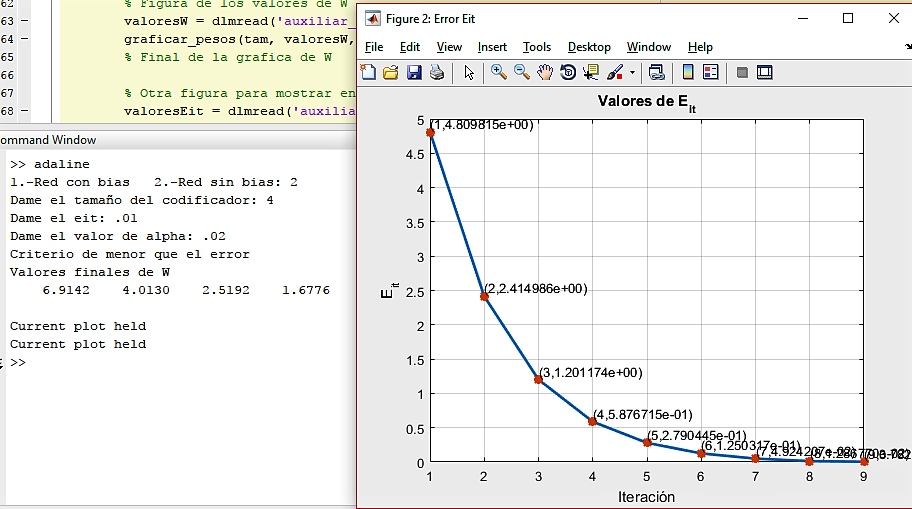
\includegraphics[width=16cm]{img/adaline3/error.png}
                    \caption{Prueba 1 de ADALINE sin bias.}
                    \label{fig:adaline3error}
                \end{center}
            \end{figure}
            
            \begin{figure}[H]
                \begin{center}
                    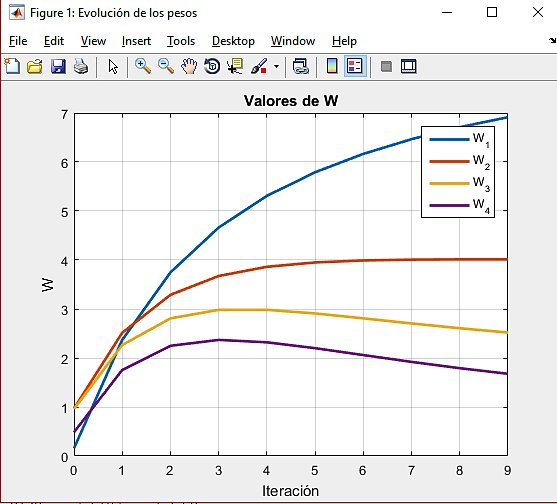
\includegraphics[width=16cm]{img/adaline3/pesosbias.png}
                    \caption{Pesos de esta prueba.}
                    \label{fig:adaline3pesos}
                \end{center}
            \end{figure}
        \textbf{Experimento 2}
        \begin{figure}[H]
            \begin{center}
                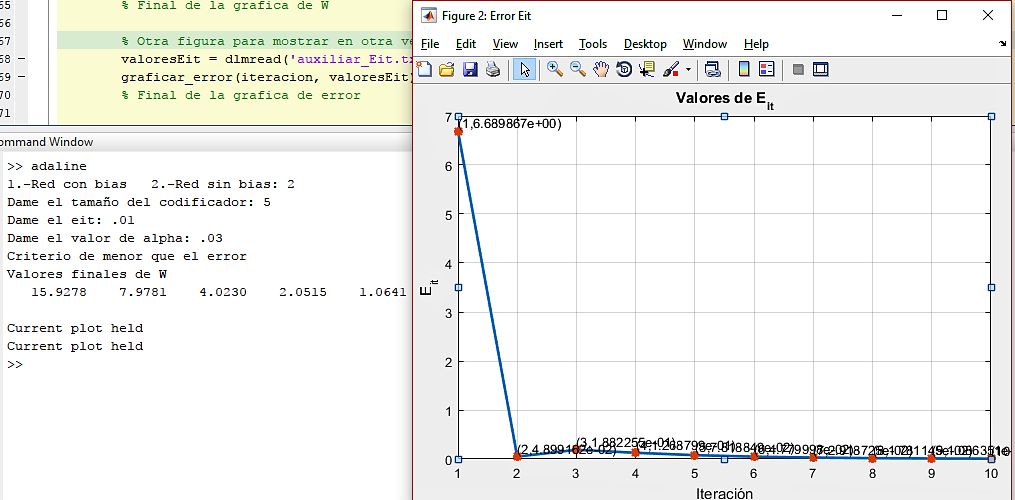
\includegraphics[width=16cm]{img/adaline4/error.png}
                \caption{Prueba 2 de ADALINE sin bias.}
                \label{fig:adaline4error}
            \end{center}
        \end{figure}
        
        \begin{figure}[H]
            \begin{center}
                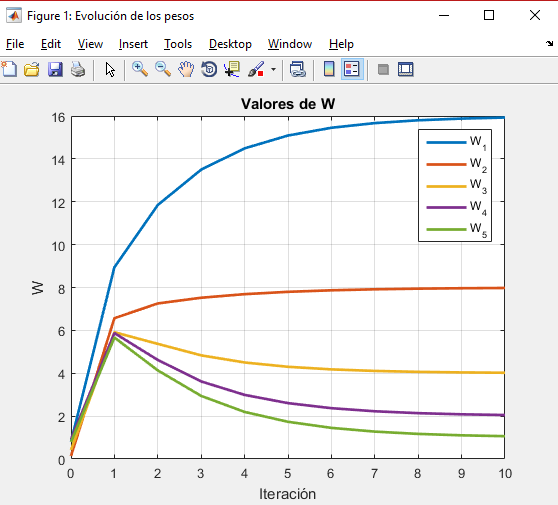
\includegraphics[width=16cm]{img/adaline4/pesosbias.png}
                \caption{Pesos de esta prueba.}
                \label{fig:adaline4pesos}
            \end{center}
        \end{figure}
    \section{Discusión de resultados}
        \subsection{Hamming}
        \subsection{Perceptron}
        \subsection{ADALINE}
    \section{Conclusiones}
    \bibliographystyle{apalike}
    \bibliography{bibliografia}
    \section{Anexo}
        En esta sección se encuentra el código de los tres programas desarrollados en MATLAB.
        \subsection{Hamming}
        \begin{lstlisting}
% Cada elemento del vector de entrada tiene solo dos posibles valores
opcion = input('Ingresa el nombre del archivo: ', 's');
archivo = dlmread(opcion);
tam = size(archivo);
% Tam de nuestros vectores prototipo
R = tam(2);

% Numero de neuronas, corresponde a cada vector prototipo
S = tam(1) - 1;

% Vector a clasificar
p = archivo(S+1, :)';

% Las filas de W1 son los vectores prototipos
% Inicializacion de W1
W1 = archivo(1:S, :);

% Cada elemento del bias es el tam del vector prototipo
% Inicializacion del bias
b1 = ones(S, 1) * R;

% Propagamos hacia adelante
a1 = purelin((W1*p)+b1);
% Fin de la capa feedforward

%Inicio de la capa recurrente
a2 = a1;
% Obtencion del valor epsilon 0 < epsilon < 1/(S-1)
epsilon = round(rand(1)*1/(S-1), 4); 
% Inicializacion y llenado de la W2 de la capa recurrente
W2 = ones(S, S);
for i = 1:S
    for j = 1:S
        if i==j
            W2(i, j) = 1;
        else
            W2(i, j) = -epsilon; 
        end;
    end;
end;

% Aqui se guardara la salida de la capa recurrente
% Metomos la salida de la capa anterior
salida = fopen('salida_hamming.txt', 'w');
fprintf(salida, '%.15f ', a2);
fprintf(salida, '\n');
% Recurrencia de la capa
t = 1;
while true
    % Obtenemos el t+1
    a2_sig = poslin(W2*a2);
    fprintf(salida, '%.15f ', a2_sig);
    fprintf(salida, '\n');
    if a2_sig == a2
        % Si ya terminamos detenemos el ciclo
        fclose(salida);
        break;
    else
        % Siguiente iteracion
        a2 = a2_sig;
    end;
    t = t + 1;
end;

% Fin de la capa recurrente
fprintf('Termino en la iteracion %d\n', t);
v = 1;
for ite = a2'
    if ite ~= 0
        break;
    else
        v = v+1;
    end;
end
fprintf('La clase a la que convergio fue: %d\n', v);
% Imprimir datos y graficar la salida de a2
a2_recurrente = dlmread('salida_hamming.txt');
figure('Name', 'Evolucion de la salida de la capa recurrente');
plot(0:t, a2_recurrente, 'LineWidth', 2);
hold;
grid;
xlabel('t');
ylabel('a^2(t)');
etiquetas = cell(1, S);
for i = 1:S
    etiquetas{i} = ['P_' num2str(i)];
end;
legend(etiquetas);
        \end{lstlisting}
        \subsection{Perceptron}
        \subsection{ADALINE}
        \begin{lstlisting}
%% Funcion principal
function adaline()
    opcion = input('1.-Red con bias   2.-Red sin bias: ', 's');
    if str2double(opcion) == 1
        adaline_bias();
    else
        % Captura de los datos
        tam = input('Dame el tam del codificador: ', 's');
        tam = str2double(tam);
        tabla_verdad = zeros(2^tam, tam+1);
        eit = input('Dame el eit: ', 's');
        eit = str2double(eit);
        alpha = input('Dame el valor de alpha: ', 's'); % 0.3
        alpha = str2double(alpha);
        N = 2^tam-1;
        W = rand(1, tam);
        auxiliar_w = fopen('auxiliar_w.txt', 'w');
        auxiliar_Eit = fopen('auxiliar_Eit.txt', 'w');
        fprintf(auxiliar_w, '%.10f ', W);
        fprintf(auxiliar_w, '\n');
        % Llenamos nuestra tabla de verdad
        for i = 0:N
            a = dec2bin(i, tam) - '0';
            tabla_verdad(i+1, 1:tam) = a;
            tabla_verdad(i+1, tam+1) = i;
        end;
        continuar = true;
        iteracion = 1;
        while continuar
            Eit = 0;
            for n = 1:N
                p = tabla_verdad(n, 1:tam)';
                a = purelin(W*p);
                t = tabla_verdad(n, tam+1);
                ed = t-a;
                Eit = Eit + ed;
                W = W + (2 * alpha * ed*p');
            end
            Eit = 1/N * Eit;
            Eit = abs(Eit);
            fprintf(auxiliar_Eit, '%.10f ', Eit);
            fprintf(auxiliar_Eit, '\n');
        
            fprintf(auxiliar_w, '%.10f ', W);
            fprintf(auxiliar_w, '\n');
            if Eit == 0
                disp('Criterio de igualdad a cero');
                break;
            elseif Eit < eit
                disp('Criterio de menor que el error');
                break;
            end
            iteracion = iteracion + 1;
        end
        fclose(auxiliar_Eit);
        fclose(auxiliar_w);
    
        % Desplegar los valores finales
        disp('Valores finales de W');
        disp(W);
        
        % Figura de los valores de W
        valoresW = dlmread('auxiliar_w.txt');
        graficar_pesos(tam, valoresW, iteracion);
        % Final de la grafica de W
        
        % Otra figura para mostrar en otra ventana
        valoresEit = dlmread('auxiliar_Eit.txt');
        graficar_error(iteracion, valoresEit)
        % Final de la grafica de error
        
        % Guardamos en un archivo
        a_final = strcat('resultado_', datestr(now, 'HH-MM_dd-mm-yyyy'));
        a_final = strcat(a_final, '.txt');
        valores_finales = fopen(a_final, 'w');
        fprintf(valores_finales, 'Valores finales de W \n');
        fprintf(valores_finales, '%.10f ', W);
        fprintf(valores_finales, '\n');
        fclose(valores_finales);
    end
end % Final de la funcion principal

%% graficar_pesos: function description
function graficar_pesos(tam, valoresW, iteracion)
    figure('Name', 'Evolucion de los pesos');
    % Grafica un vector en x y otro vector en y
    plot(0:iteracion, valoresW, 'LineWidth', 2); 
    hold;
    grid;
    % Etiquetas de los ejes
    xlabel('Iteracion');
    ylabel('W');
    
    % Titulo de nuestra grafica
    etiquetas = cell(1, tam);
    for i = 1:tam
        etiquetas{i} = ['W_' num2str(i)];
    end;
    legend(etiquetas);
    title('Valores de W');
end

%% graficar_error: function description
function graficar_error(iteracion, valoresEit)
    figure('Name', 'Error Eit');
    x = 1:iteracion;
    % Grafica un vector en x y otro vector en y
    plot(x, valoresEit, 'LineWidth', 2);
    hold;
    plot(x, valoresEit, '*', 'LineWidth', 2);
    grid;
    % Imprime las coordenadas de Eit
    strValues = strtrim(cellstr(num2str([x(:) valoresEit(:)], '(%d,%d)')));
    text(x, valoresEit, strValues, 'VerticalAlignment', 'bottom');
    % Etiquetas de los ejes
    xlabel('Iteracion');
    ylabel('E_{it}');
    % Titulo de nuestra grafica
    title('Valores de E_{it}');
end

%Con bias
function adaline_bias()
    archivo = input('Dame el nombre del archivo: ', 's');
    prueba = fopen(archivo, 'r');
    S = 0;
    targets = [];
    prototipos = [];
    R = 0;
    dimen = [];
    tipo_lectura = 0;
    while feof(prueba) == 0
        linea = fgetl(prueba);
        if linea ~= '{'
            fclose(prueba);
            datos = dlmread(archivo);
            tam = size(datos);
            S = 1;
            prototipos = datos(:, 1:tam(2)-1)';
            dimen = size(prototipos);
            targets = datos(:, tam(2))';
            R = dimen(1);
            tipo_lectura = 1;
            break;
        else
            linea = linea(2:length(linea)-1);
            proto = linea(2:find(linea==',')-2);
            tar = linea(find(linea==',')+2:length(linea)-1);
            proto = str2num(proto);
            tar = str2num(tar);
            prototipos = [prototipos proto'];
            targets = [targets tar'];
        end
    end
    if tipo_lectura == 0
        S = 2;
        dimen = size(prototipos);
        R = dimen(1);
    end   
    itmax = input('Ingrese valor de itmax: ', 's'); %5
    itmax = str2double(itmax);
    alpha = input('Dame el valor de alpha: ', 's'); % 0.3
    alpha = str2double(alpha);
    eit = input('Dame el eit: ', 's');
    eit = str2double(eit);
    W = ones(S, R);
    b = ones(S, 1);
    
    auxiliar_w = fopen('auxiliar_w.txt', 'w');
    auxiliar_bias = fopen('auxiliar_bias.txt', 'w');
    auxiliar_error = fopen('auxiliar_Eit.txt', 'w');
    fprintf(auxiliar_w, '%.10f ', W);
    fprintf(auxiliar_w, '\n');
    
    fprintf(auxiliar_bias, '%.10f ', b);
    fprintf(auxiliar_bias, '\n');
    criterio = 0;
    for iteracion = 1:itmax
        Eit = 0;
        for n = 1:dimen(2)
            p = prototipos(:, n);
            a = purelin(W*p + b);
            t = targets(:, n);
            ed = t-a;
            Eit = Eit + ed;
            W = W + (2 * alpha * ed * p');
            b = b + (2 * alpha * ed);
        end
        Eit = 1/dimen(2) * Eit;
        Eit = abs(Eit);
        fprintf(auxiliar_error, '%.10f ', Eit);
        fprintf(auxiliar_error, '\n');
        
        fprintf(auxiliar_w, '%.10f ', W);
        fprintf(auxiliar_w, '\n');
        
        fprintf(auxiliar_bias, '%.10f ', b);
        fprintf(auxiliar_bias, '\n');
        if Eit == 0
            criterio = 1;
            break;
        elseif Eit < eit
            criterio = 2;
            break;
        end
    end
    fclose(auxiliar_error);
    fclose(auxiliar_w);
    fclose(auxiliar_bias);
    
    % Figura de los valores de W
    valoresW = dlmread('auxiliar_w.txt');
    valores_bias = dlmread('auxiliar_bias.txt');
    graficar_pesos_bias(valoresW, iteracion, S, R);
    graficar_bias(valores_bias, iteracion, S);
    % Final de la grafica de W
    
    % Otra figura para mostrar en otra ventana
    valoresEit = dlmread('auxiliar_Eit.txt');
    graficar_error_bias(iteracion, valoresEit, S);
    % Final de la grafica de error
    
    if criterio == 0
        disp('Termino alcanzando el maximo de iteraciones')
    elseif criterio == 1
        disp('Termino por criterio de error igual a 0');
        fprintf('Termino en la iteracion %d\n', iteracion);
        disp('Valores finales de W:');
        disp(W);
        disp('Valores finales del bias:');
        disp(b);
    else
        disp('Termino por criterio de menor al error permitido');
        fprintf('Termino en la iteracion %d\n', iteracion);
        disp('Valores finales de W:');
        disp(W);
        disp('Valores finales del bias:');
        disp(b);
    end
    
    archivo_final = strcat('resultado_', datestr(now, 'HH-MM_dd-mm-yyyy'));
    archivo_final = strcat(archivo_final, '.txt');
    finales = fopen(archivo_final, 'w');
    fprintf(finales, 'Valores finales de W: \n');
    fprintf(finales, '%.10f ', W);
    fprintf(finales, '\n');
    
    fprintf(finales, 'Valores finales del bias: \n');
    fprintf(finales, '%.10f ', b);
    fprintf(finales, '\n');
    fclose(finales);
end


%% graficar_pesos: function description
function graficar_pesos_bias(valoresW, iteracion, S, R)
    figure('Name', 'Evolucion de los pesos');
    % Grafica un vector en x y otro vector en y
    plot(0:iteracion, valoresW, 'LineWidth', 2); 
    hold;
    grid;
    % Etiquetas de los ejes
    xlabel('Iteracion');
    ylabel('W');
    
    etiquetas = cell(1, S*R);
    k = 1;
    for i = 1:S
        for j = 1:R
            etiquetas{k} = ['W_{' num2str(i) ',' num2str(j) '}'];
            k = k+1;
        end;
    end;
    legend(etiquetas);
    title('Valores de W');
end

%% graficar_error: function description
function graficar_error_bias(iteracion, valoresEit, S)
    figure('Name', 'Error Eit');
    x = 1:iteracion;
    % Grafica un vector en x y otro vector en y
    plot(x, valoresEit, 'LineWidth', 2);
    hold;
    grid;
    % Etiquetas de los ejes
    xlabel('Iteracion');
    ylabel('E_{it}');
    % Titulo de nuestra grafica
    etiquetas = cell(1, S);
    for i = 1:S
        etiquetas{i} = ['Neurona ' num2str(i)];
    end;
    legend(etiquetas);
    % Titulo de nuestra grafica
    title('Valores de E_{it}');
end

%% graficar_bias
function graficar_bias(valores_bias, iteracion, S)
    figure('Name', 'Evolucion del bias');
    % Grafica un vector en x y otro vector en y
    plot(0:iteracion, valores_bias, 'LineWidth', 2); 
    hold;
    grid;
    % Etiquetas de los ejes
    xlabel('Iteracion');
    ylabel('Bias');
    % Titulo de nuestra grafica
    etiquetas = cell(1, S);
    for i = 1:S
        etiquetas{i} = ['b_' num2str(i)];
    end;
    legend(etiquetas);
    title('Valores del bias');
end
        \end{lstlisting}
\end{document}